\section{Physical quality of the matched generators}\label{app:generator-quality}
We score the 16,384 saved 128-call outputs from Section~\ref{sec:matched-generators}, without retraining or changing coordinates. The evaluation protocol is fixed before scoring. eSEN evaluates every output and its reflection, requiring 33,024 calls. GFN2 evaluates graph-valid outputs and both reference inversions; all 2,198 calculations succeed, including 256 reference checks.

Joint yield counts outputs passing graph validity and a force threshold over all attempts. Figure~\ref{fig:generator-quality} varies the threshold to show sensitivity to this choice. A force cutoff measures residual-force quality, not stationarity. These models share the architecture and training budget in Appendix~\ref{app:matched-generators} and receive no physical updates.

\begin{figure}[htbp]
\centering
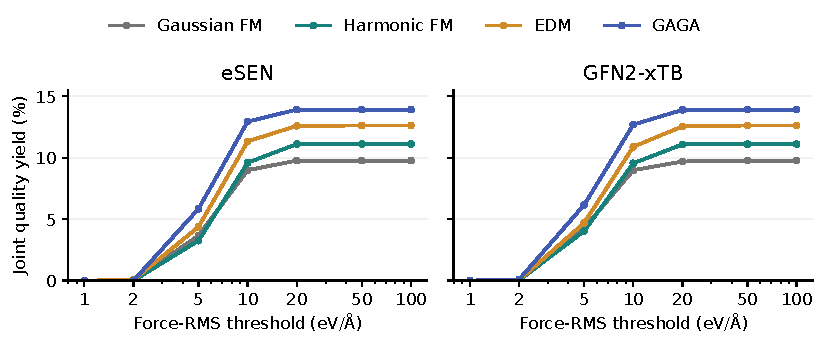
\includegraphics[width=\linewidth]{../research/figures/final_complete_v1/figures/quality_yield.pdf}
\caption{Joint yield versus force threshold, pooling two initializations and 64 compositions. All attempts contribute to the denominator. GAGA has the highest pooled yield at most nontrivial thresholds under both potentials.}\label{fig:generator-quality}
\end{figure}

\begin{table}[htbp]
\centering
\caption{GFN2 scores of matched generators. Energy and force are medians over each method's graph-valid outputs; yield uses all 4,096 attempts. Energy excess is relative to one same-composition OMol25 reference, whose connectivity may differ from the generated graph.}
\small
\begin{tabular}{lrrr}
\toprule
Method & Energy excess (eV/atom) & Force RMS (eV/\AA) & Yield at 5 eV/\AA\ (\%)\\
\midrule
Gaussian FM & 0.6820 & 5.2911 & 4.27\\
Harmonic FM & 0.7114 & 5.8183 & 4.03\\
EDM & 0.6799 & 5.8768 & 4.69\\
GAGA & 0.6604 & 5.2785 & 6.15\\
\bottomrule
\end{tabular}
\end{table}

GAGA has the stronger pooled physical scores in this matched comparison. The harmonic source improves graph validity without improving physical scores among valid outputs. The physical-adaptation studies separately test whether local force targets address this gap.
